%
%  kant.two
%
%  Created by Mark Eli Kalderon on 2007-08-04.
%  Copyright (c) 2007 Mark Eli Kalderon. All rights reserved.
%
%  Beamer

% Definitions and macros
\newcommand{\change}{\textcolor{blue}{\textbf{CHANGE SLIDE}}}
\def\myauthor{Mark Eli Kalderon} 
\def\mytitle{Introduction to Moral Philosophy}
\def\mysubtitle{Kant}
\def\myinstitution{University College London}
\def\myurl{http://markelikalderon.com/teaching/}

% Packages specific to lecture notes
\mode<article>{
	\usepackage{palatino}
}

% Packages specific to beamer presentation
\mode<presentation>{
	\usetheme{Darmstadt}
	\setbeamercovered{transparent}
	\pgfdeclareimage[height=0.5cm]{university-logo}{../../../Graphics/logo_sml_blk}
	\logo{\pgfuseimage{university-logo}}
}

% Packages common to lecture notes and beamer presentation
\usepackage{pgf}
\usepackage{tikz}
\usepackage{hyperref}

\setjobnamebeamerversion{kant.two.beamer}

\title{\mytitle}
\subtitle{\mysubtitle}

\author{\myauthor\\
\url{\myurl}}
\institute{\myinstitution}

% \date[Short Occasion] % (optional)
% {Date / Occasion}

\begin{document}

\frame{\maketitle}

\section{The Good Will and Duty}\label{sec:the_good_will_and_duty} % (fold)

\change\ Kant proposes to ``explicate'' the concept of \emph{the good will}. He does so by considering the related concept of \emph{duty} ``which contains that of a good will though under certain subjective limitations and hindrances, which, however, far from concealing it and making it unrecognizable, rather bring it out by contrast and make it shine forth all the more brightly'' (G 4:397). Two observations can be made about this.

First, the concept of the good will is broader than the concept of a will that acts from duty: Kant claims that the concept of duty ``contains'' the concept of the good will. So Kant is proposing that we consider only special cases of the good will, i.e., cases where the good will must overcome ``certain subjective limitations and hindrances''. So acting from duty is not a necessary condition for possessing a good will. A will can be good even when it does not act from duty (as when no duty applies in a given circumstance).

Second, Kant considers these special cases of the good will where the good will must overcome ``certain subjective limitations and hindrances'' in order that the absolute value of the good will ``shine forth all the more brightly'' to common rational moral cognition. The idea is that in considering the good will under ``certain subjective limitations and hindrances'' its value will be clearly distinguished and recognized to be incomparably higher than the value of any gift of nature or fortune such as, for example, being naturally endowed with a sympathetic temperament.

Kant distinguishes \emph{acting in conformity with duty} from \emph{acting from duty}.

An action conforms to duty just in case it is compatible with what duty requires. Notice that in order for an action to conform to duty it is only necessary that an action be compatible with the requirements of duty no matter what the motive was for performing that action. So, for example, if it is a duty to be honest in commercial transactions, the actions of shopkeeper who charges a fixed regular price for everyone conforms to duty even if he is motivated to do so out of rational self-interest rather than respect for the moral law.

In order for an action to be done from duty, not only must it conform to duty (not only must it be compatible with what duty requires), but it must also be motivated in a certain way. Actions done from duty must be done for the sake of duty and not for the sake of any nonmoral incentive, such as rational self-interest. \change

% \textbf{See Figure~\ref{fig:slide1}.}
% 
% \begin{figure}[ht]
%     \begin{center}
%         \includeslide[height=5cm]{../Presentation/slide1<1>}
%     \end{center}
%     \caption{Acting in Conformity with Duty vs Acting from Duty}
%     \label{fig:slide9}
% \end{figure}

\frame<presentation>[label=slide1]{
    \frametitle{Acting in Conformity with Duty vs Acting from Duty}
        \begin{columns}
            \begin{column}{3cm}
                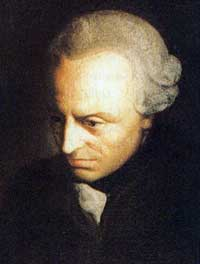
\includegraphics[height=4cm]{../../../graphics/kant.jpg}
            \end{column}
            \begin{column}{7cm}
                \begin{itemize}
                    \item If a person \alert{conforms to duty}, then his actions are compatible with what duty requires no matter what their motivation
                    \item If a person \alert{acts from duty}, not only must his actions be compatible with what duty requires, but they must be motivated in a certain way---for the sake of duty as opposed to rational self-interest
                \end{itemize}
            \end{column}
        \end{columns}
}

Kant claims that only actions done from duty have \emph{moral worth} or \emph{moral content}.

This is not to claim that actions in conformity with duty but not done from duty have no moral value. That such actions fulfill the requirements of duty is morally valuable and so merit moral approval. Indeed such actions might even merit ``praise and encouragement'' just in virtue of conforming to duty even if they were not done from duty (G 4:398).

The moral worth of an action goes beyond the value that would merit moral approval. The moral worth of an action is more than its compatibility with the requirements of duty. The moral worth of an action consists in its being motivated in the right sort of way. Specifically, an action only has moral worth if it is done solely from duty. Thus, the moral worth of an action merits not \emph{approval} but \emph{esteem}. Esteem is the recognition of the special worth of a character that is a gift of neither nature nor fortune. Not all actions of a good will merit esteem, only those that are done solely from duty in the absence of any other incentive. \change

% \textbf{See Figure~\ref{fig:slide2}.}
% 
% \begin{figure}[ht]
%     \begin{center}
%         \includeslide[height=5cm]{slide2<1>}
%     \end{center}
%     \caption{The Moral Worth of Acting from Duty}
%     \label{fig:slide10}
% \end{figure}

\frame<presentation>[label=slide2]{
    \frametitle{The Moral Worth of Acting from Duty}
        \begin{columns}
            \begin{column}{3cm}
                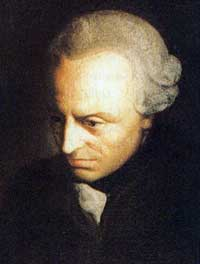
\includegraphics[height=4cm]{../../../graphics/kant.jpg}
            \end{column}
            \begin{column}{7cm}
                \begin{itemize}
                    \item Only actions done from duty have \alert{moral worth} or \alert{moral content}
                    \item The value of acting from duty foes beyond the value of acting in conformity with duty. While the latter merits \alert{moral approval}, the former merits \alert{esteem}
                    \item \alert{Esteem} is the recognition of a special worth of character that is neither a gift of nature nor fortune
                \end{itemize}
            \end{column}
        \end{columns}
}

Inclination plays an important role in Kant’s subsequent discussion so it will be helpful to understand what Kant means by ``inclination''.

In a footnote, Kant defines inclination as ``the dependence of the faculty of desire on feeling'' (G 4:414n). This is not terribly helpful, but, in later work, Kant explains further.

According to Kant, the mind’s powers divide into three faculties:

\begin{enumerate}
	\item The faculty of cognition
	\item The faculty of feeling
	\item The faculty of desire
\end{enumerate}

The faculty of desire is the mind’s capacity to produce an object by means of a representation. Desiring an object involves having a representation of an object accompanied by a feeling pleasure. In contrast, an aversion involves a representation of an object accompanied by a feeling of displeasure. In empirical desire or aversion, the feeling of pleasure or displeasure is the contingent result of the way in which the representation of the object affects one’s susceptibility to feeling. When an empirical desire becomes habitual, it is an inclination. When an empirical aversion becomes habitual, it is fear.

Following Hume, Kant holds that the regular operation of habit occurs unreflectively. However, when a person reflects and judges that pleasure is regularly connected with an object, a person takes an interest in that object. Thus awareness of an inclination produces an interest in the object (G 4:413). When an interest arises from inclination it is a \emph{pathological interest}. Interest, however, can arise from rational grounds as well. When it does, it is a \emph{practical interest}. In the case of practical interest, a person takes an interest in an object even if he does not act from interest (G 4:413). \change

% \textbf{See Figure~\ref{fig:slide3}.}
% 
% \begin{figure}[ht]
%     \begin{center}
%         \includeslide[height=5cm]{slide3<1>}
%     \end{center}
%     \caption{Inclination}
%     \label{fig:slide11}
% \end{figure}

\frame<presentation>[label=slide3]{
    \frametitle{Inclination}
        \begin{columns}
            \begin{column}{3cm}
                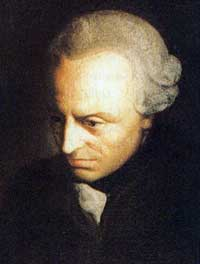
\includegraphics[height=4cm]{../../../graphics/kant.jpg}
            \end{column}
            \begin{column}{7cm}
                \begin{itemize}
                    \item The \alert{faculty of desire} is the mind's capacity to produce an object by means of a representation. \alert{Desiring an object} involves a representation of the object accompanied by a feeling of pleasure
                    \item In \alert{empirical desire}, the feeling of pleasure is the contingent result of the way in which the representation of the object affects one's susceptability to feeling
                    \item When an empirical desire becomes habitual, it becomes an \alert{inclination}
                \end{itemize}
            \end{column}
        \end{columns}
}

In the first section, Kant puts forward three important propositions about duty:
\begin{enumerate}
    \item An action has moral worth only when it is done from duty.
    \item ``An action from duty has its moral worth not in the purpose to be attained by it but in the maxim in accordance with which it is decided upon, and therefore does not depend upon the realization of the object of the action but merely upon the principle of volition in accordance with which the action is done without regard for an object of the faculty of desire.''  (G 4:399-400)
    \item ``Duty is the necessity of an action from respect for law.'' (G 4:400)
\end{enumerate}
While the content of the first proposition is relatively clear, the content of the second and third propositions need further explanation. Each of Kant's three propositions are justified on the basis of material culled from common rational moral cognition. Reflection upon the third proposition leads to the first formulation of the categorical imperative. \change

% \textbf{See Figure~\ref{fig:slide4}.}
% 
% \begin{figure}[ht]
%     \begin{center}
%         \includeslide[height=5cm]{slide4<1>}
%     \end{center}
%     \caption{Kant's Three Propositions}
%     \label{fig:slide12}
% \end{figure}

\frame<presentation>[label=slide4]{
    \frametitle{Kant's Three Propositions}
        \begin{columns}
            \begin{column}{3cm}
                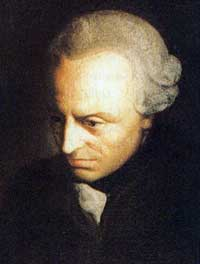
\includegraphics[height=4cm]{../../../graphics/kant.jpg}
            \end{column}
            \begin{column}{7cm}
                \begin{enumerate}
                    \item An action has moral worth only when it is done from duty.
                    \item ``An action from duty has its moral worth not in the purpose to be attained by it but in the maxim in accordance with which it is decided upon, and therefore does not depend upon the realization of the object of the action but merely upon the principle of volition in accordance with which the action is done without regard for an object of the faculty of desire.''  (G 4:399-400)
                    \item ``Duty is the necessity of an action from respect for law.'' (G 4:400)
                \end{enumerate}
            \end{column}
        \end{columns}
}

% section the_good_will_and_duty (end)

\section{Kant's Three Propositions}\label{sec:kant_s_three_propositions} % (fold)

Kant's first important claim about duty is:

\begin{quote}
	An action has moral worth only when it is done from duty.
\end{quote}

Kant seeks to elicit common rational moral cognition's assent to this proposition by considering its reaction to four examples. The first example is that of a shopkeeper who has no immediate inclination to not overcharge an inexperienced customer (which is his duty) but conforms his actions to duty out of self-interest, to avoid a bad reputation (G 4:397). The three following examples all involve comparing two cases where a person performs an action required by duty (preserving one's life, acting beneficently towards those in need, promoting one's own happiness) (G 4:397--399). In the first case, the person performs the action because of an immediate inclination to do so (self-preservation, sympathy, and self love). In the second case, the person performs the action because it is his duty. In each of the cases of acting from duty, the person either must overcome some opposing inclination or must at least act without the help of inclination. Kant's idea is that while the first of these cases where action conforms to duty but is motivated by an immediate inclination, will elicit approval from common rational moral cognition, the second of these case, where duty is the sole motive, will elicit esteem. Recall, esteem is only merited by the moral worth of an action. So, if common rational moral cognition esteems only actions done from duty, this is good evidence that common rational moral cognition is committed to an action having moral worth only when it is done from duty. \change

% \textbf{See Figure~\ref{fig:slide5}.}
% 
% \begin{figure}[ht]
%     \begin{center}
%         \includeslide[height=5cm]{slide5<1>}
%     \end{center}
%     \caption{Kant's First Proposition}
%     \label{fig:slide1}
% \end{figure}

\begin{frame}<presentation>[label=slide5]
    \frametitle{Kant's First Proposition}
        \begin{columns}
            \begin{column}{3cm}
                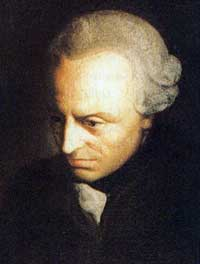
\includegraphics[height=4cm]{../../../graphics/kant.jpg}
            \end{column}
            \begin{column}{7cm}
                \begin{block}{Kant's First Proposition}
                    An action has moral worth only when it is done from duty.
                \end{block}
            \end{column}
        \end{columns}
\end{frame}

Notice that the cases that elicit esteem are those in which the person acts from duty even though there is no inclination to do so or a strong inclination to act contrary to duty. Thus if Kant held that a good will only ever acts from duty, he would be committed to claiming that a person only ever has a good will when he lacks a nonmoral incentive to do his duty. If we further assume that we should strive to have a good will this would commit Kant to holding that we should strive to eliminate all nonmoral incentives to do our duty. This line of thought is plausibly the source of Schiller's satire:

\begin{quote}
    \emph{Scruples of Conscience}\\
	I like to serve my friends, but unfortunately I do it by inclination And so I am bothered by the thought that I am not virtuous.\\
	\emph{Decision}\\
	There is no other way but this! You must seek to despise them And do with repugnance what duty bids you.
\end{quote}

Kant, however, explicitly denies these commitments. Kant does not believe that we should strive to eliminate all nonmoral incentives to do our duty. Rather, Kant explicitly claims that we have a duty to cultivate love, sympathy, and other inclinations that make it easier to do our duty (MS 6:456-7). Moreover, Kant denies that actions done from duty are done ``with repugnance''. Conforming to duty with repugnance reveals ``a hidden hatred of the law'' and is the opposite of acting with a good will (R 6:24n). The line of thought leading to Schiller's satire goes wrong at the very first step. It is not the case that a good will only ever acts from duty. A person can possess a good will even in circumstances where no duty applies to his action. Moreover, a divine will is a good will even though it is impossible for it to act from duty (since being infinite in nature it is not subject to the ``subjective limitations and hindrances'' of finite beings). \change

% \textbf{See Figure~\ref{fig:slide6}.}
% 
% \begin{figure}[ht]
%     \begin{center}
%         \includeslide[height=5cm]{slide6<1>}
%     \end{center}
%     \caption{Schiller's Satire}
%     \label{fig:slide2}
% \end{figure}

\begin{frame}<presentation>[label=slide6]
    \frametitle{Schiller's Satire}
        \begin{columns}
            \begin{column}{3cm}
                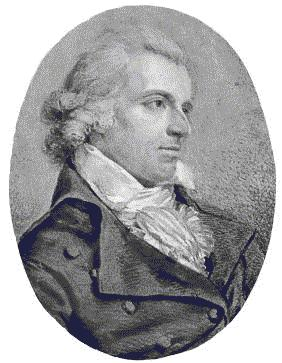
\includegraphics[height=4cm]{../../../graphics/schiller.jpg}
            \end{column}
            \begin{column}{7cm}
                \begin{quote}
                    \alert{Scruples of Conscience}\\
                	I like to serve my friends, but unfortunately I do it by inclination And so I am bothered by the thought that I am not virtuous.\\
                	\alert{Decision}\\
                	There is no other way but this! You must seek to despise them And do with repugnance what duty bids you.
                \end{quote}
            \end{column}
        \end{columns}
\end{frame}

Kant's second important claim about duty is:

\begin{quote}
	An action from duty has its moral worth not in the purpose to be attained by it but in the maxim in accordance with which it is decided upon, and therefore does not depend upon the realization of the object of the action but merely upon the principle of volition in accordance with which the action is done without regard for an object of the faculty of desire. (G 4:399-400)
\end{quote}

Kant's second proposition is really two claims in one. The first claim is negative and the second claim is positive:

\begin{enumerate}
	\item The moral worth of an action done from duty does not depend on what it accomplishes.
	\item The moral worth of an action done from duty depends merely on its ``maxim'' or ``principle of volition''.
\end{enumerate}

The first, negative claim clearly parallel's a negative claim about the good will: Just as the value of a good will does not depend on what it accomplishes, so the moral worth of an action does not depend on what it accomplishes. This should not be surprising since the concept of duty ``contains'' the concept of a good will. Kant says that the negative claim ``is clear from what has gone on before''. Kant is partly alluding to the parallel discussion of the good will and partly alluding to the discussion of the four examples. Suppose in acting in conformity with duty a person's action accomplishes some purpose he is inclined to. According to Kant, this elicits from common rational moral cognition only approval. But in acting solely from duty a person's action accomplishes no purpose he is inclined to. According to Kant, this elicits from common rational moral cognition not approval but esteem. Since esteem is only merited by the moral worth of an action, it follows that the moral worth of an action does not depend on accomplishing some inclined purpose.

If the moral worth of an action does not depend on what it accomplishes, then what does it depend upon? According to Kant, the moral worth of an action depends on its ``maxim'' or ``principle of volition''. Kant's argument is abstract here:

\begin{quote}
	In what, then, can this worth lie, if it is not to be in the will in relation to the hoped for effect of the action? It can lie nowhere else than in the principle of the will without regard for the ends that can be brought about by such an action. For, the will stands between its a priori principle, which is formal, and its a posteriori incentive, which is material, as at a crossroads; and since it must still be determined by something, it must be determined by the formal principle of volition \ldots (G 4:400)
\end{quote}

The point can be put less abstractly by following Kant's discussion of the four examples. When common rational moral cognition esteems an action done from duty, this esteem is merited by the fact that the person acted from duty in the absence of supporting inclination and potentially in the face of opposing inclination. What merits esteem is that the person freely chose to do his duty despite ``certain subjective limitations and hindrances'' (G 4:397). It is the policy or ``maxim'' that he adopted, to do what duty requires, that elicits esteem from common rational moral cognition and not the accomplishment of any inclined purpose. So it can only be in the maxim of the action that its moral worth resides. \change

% \textbf{See Figure~\ref{fig:slide7}.}
% 
% \begin{figure}[ht]
%     \begin{center}
%         \includeslide[height=5cm]{slide7<1>}
%     \end{center}
%     \caption{Kant's Second Proposition}
%     \label{fig:slide3}
% \end{figure}

\begin{frame}<presentation>[label=slide7]
    \frametitle{Kant's Second Proposition}
        \begin{columns}
            \begin{column}{3cm}
                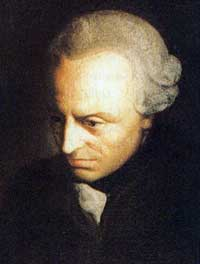
\includegraphics[height=4cm]{../../../graphics/kant.jpg}
            \end{column}
            \begin{column}{7cm}
                \begin{block}{Kant's Second Proposition}
                	An action from duty has its moral worth not in the purpose to be attained by it but in the maxim in accordance with which it is decided upon, and therefore does not depend upon the realization of the object of the action but merely upon the principle of volition in accordance with which the action is done without regard for an object of the faculty of desire. (G 4:399--400)
                \end{block}
                
            \end{column}
        \end{columns}
\end{frame}

Kant's third important claim about duty is:

\begin{quote}
	Duty is the necessity of an action from respect for law. (G 4:400)
\end{quote}

Kant claims that his third proposition follows from the previous two. Strictly speaking this cannot be right, since the third proposition involves the notion of respect not mentioned in the first two propositions. However, the third proposition plausibly follows from the first two propositions in conjunction with a positive characterization of respect.

Kant claims that acting from duty involves the feeling of respect for the moral law. The feeling of respect arises from the:

\begin{quote}
	Immediate determination of the will by means of the law and consciousness of this... (G 4:401n)
\end{quote}

\emph{Respect}, unlike self-preservation, sympathy and self-love, is not an inclination. In acting from inclination, a person attempts to achieve some purpose because he antecedently wants to. But a person respects something not because he wants to respect it. Rather, a person respects something because he recognizes the reasons he must respect it. Thus Kant claims that ``only what is connected with my will merely as a ground and never as an effect...can be an object of respect \ldots'' (G 4:400). This is because respect essentially involves reasons that are potentially distinct from any purpose of inclination that might be achieved by acting. In acting from duty, a person does his duty, not because he antecedently wants to. Rather, in acting from duty, a person does his duty because he recognizes the reasons he must. This is because acting from duty essentially involves reasons that are potentially distinct from any purpose of inclination. From this, Kant concludes that in acting from duty a person manifests respect for the moral law. Notice that the object of respect is the moral law. In Kant's sense of the term, one can only respect a person derivatively, as ``an example of the moral law'' (G 4:401n), that is, as an esteemable exemplar of someone who consciously submits their will to the moral law. In claiming that ``duty is the necessity of an action from respect for the moral law'', Kant claims that in acting from duty a person's will is wholly determined by a conscious representation of the moral law and is thus accompanied by a feeling of respect. \change

% \textbf{See Figure~\ref{fig:slide8}.}
% 
% \begin{figure}[ht]
%     \begin{center}
%         \includeslide[height=5cm]{slide8<1>}
%     \end{center}
%     \caption{Kant's Third Proposition}
%     \label{fig:slide8}
% \end{figure}

\begin{frame}<presentation>[label=slide8]
    \frametitle{Kant's Third Proposition}
        \begin{columns}
            \begin{column}{3cm}
                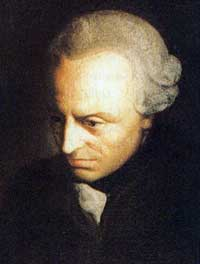
\includegraphics[height=4cm]{../../../graphics/kant.jpg}
            \end{column}
            \begin{column}{7cm}
                \begin{block}{Kant's Third Proposition}
                	Duty is the necessity of an action from respect for law. (G 4:400)
                \end{block}
            \end{column}
        \end{columns}
\end{frame}

Kant's discussion of duty leads him to pose the following question:

\begin{quote}
	But what kind of law can that be, the representation of which must determine the will, even without regard for the effect expected from it, in order for the will to be called good absolutely and without limitation? (G 4:402)
\end{quote}

Kant's answer to this question is breathtaking in its brevity and import for in his answer Kant claims to have discovered a provisional formulation of the supreme principle of morality:

\begin{quote}
	Since I have deprived the will of every impulse that could arise for it from obeying some law, nothing is left but the conformity of actions as such with universal law, which alone is to serve the will as its principle, that is, I ought never to act except in such a way that I could also will that my maxim should become a universal law. (G 4:402)
\end{quote}

This is the \textbf{Formula of Universal Law}, a variant of the first of the three formulations of the categorical imperative. \change

% \textbf{See Figure~\ref{fig:slide9}.}
% 
% \begin{figure}[ht]
%     \begin{center}
%         \includeslide[height=5cm]{slide9<1>}
%     \end{center}
%     \caption{First Derivation of the Categorical Imperative}
%     \label{fig:slide5}
% \end{figure}

\begin{frame}<presentation>[label=slide9]
    \frametitle{First Derivation of the Categorical Imperative}
        \begin{columns}
            \begin{column}{3cm}
                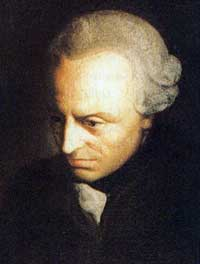
\includegraphics[height=4cm]{../../../graphics/kant.jpg}
            \end{column}
            \begin{column}{7cm}
                \begin{quote}
                	Since I have deprived the will of every impulse that could arise for it from obeying some law, nothing is left but the conformity of actions as such with universal law, which alone is to serve the will as its principle, that is, I ought never to act except in such a way that I could also will that my maxim should become a universal law. (G 4:402)
                \end{quote}
            \end{column}
        \end{columns}
\end{frame}

Schopenhauer, in \emph{On the Basis of Morality}, criticizes the argument as follows:

\begin{quote}
	By disdaining all empirical motives of the will Kant removed as empirical everything objective and everything subjective on which a law for the will could be based. And so for the substance of that law he had nothing left but its own form. Now this is simply conformity to law; but such conformity consists in its being applicable to all and so in its universal validity. Accordingly this becomes the substance and consequently the purport and meaning of the law are nothing but its universal validity itself. It will therefore read ``Act only in accordance with that maxim which you can at the same time wish will become a universal law for all rational beings'' \ldots\ I pay a tribute of sincere admiration to the great ingenuity with which Kant performed this trick.
\end{quote}

Schopenhauer complains that the inference from ``conformity of actions as such with universal law'' to the Formula of Universal Law is fallacious. Kant reasons from the universal applicability of the law, its validity for all rational beings, to the content of the law. But the content of the law, as represented by the Formula of Universal Law, goes beyond its universal applicability for it contains, in addition, the idea that ``I could also will that my maxim should become a universal law''. But we have so far been given no reason to think that the universal applicability of a law necessarily involves what we could or could not will.

It is plausible that Kant is anticipating here. If rational beings are the authors of universal law, then the universal applicability of the law, its validity for all rational beings, would necessarily involve what a rational being could or could not will. Kant is thus anticipating the idea of autonomy introduced in the second section. Perhaps a claim about autonomy is functioning as a suppressed premise. Unfortunately, the justification for any such claim is based on the philosophical arguments of the second section. This means that Kant cannot rely on philosophical claims about autonomy in the first section since in the first section he is limiting himself to claims that can be elicited from common rational moral cognition.

Perhaps Kant's reasoning is nondemonstrative here. While he cannot demonstrate that the Formula of Universal Law follows from its universal applicability solely from premises that can be elicted from common rational moral cognition, Kant might be exercising Socratic influence here. Perhaps he thinks he need only explicitly state the Formula of Universal Law for common rational cognition to recognize it as a representation of the practical principle that it unreflectively adheres to. \change

% \textbf{See Figure~\ref{fig:slide10}.}
% 
% \begin{figure}[ht]
%     \begin{center}
%         \includeslide[height=5cm]{slide10<1>}
%     \end{center}
%     \caption{Schopenhauer's Criticism}
%     \label{fig:slide6}
% \end{figure}

\begin{frame}<presentation>[label=slide10]
    \frametitle{Schopenhauer's Criticism}
        \begin{columns}
            \begin{column}{3cm}
                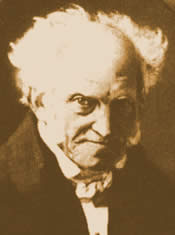
\includegraphics[height=4cm]{../../../graphics/schopenhauer.jpg}
            \end{column}
            \begin{column}{7cm}
                \begin{quote}
                	I pay a tribute of sincere admiration to the great ingenuity with which Kant performed this trick.
                \end{quote}
            \end{column}
        \end{columns}
\end{frame}

Kant's avowed purpose in discussing duty was to ``explicate'' the concept of the good will ``that is to be esteemed in itself and is good apart from any further purpose'' (G 4:397). To what extent has that purpose been achieved?

In acting in such a way that he could also will that his maxim be a universal law, a person acts out of respect for the law. Kant writes:

\begin{quote}
	Though I do no yet see what this respect is based upon (this the philosopher may investigate), I at least understand this much; that it is an estimation of a worth that far outweighs any worth of what is recommended by inclination, and that the necessity of my action from pure respect for the practical law is what constitutes duty, to which every other motive must give way because it is the condition of a will good in itself, the worth of which surpasses all else. (G 4:403)
\end{quote}

Kant's point is this: The unconditional value of the good will, a value that is incomparably higher than the value of any gift of nature or fortune, is manifest in its capacity to be immediately determined by the moral law without supporting inclination or even in the face of opposing inclination.

Kant underscores this by contrasting the value of innocence and goodness (a normative contrast that he inherits from Rousseau). Though innocence enjoys a kind of splendor and is an object of nostalgia when it passes, it exists in fragile harmony with what duty requires and is easily seduced. An innocent human being's conformity to duty is contingent and is easily interfered with by the ``counterweight of his needs and inclinations, the entire satisfaction of which he sums up under the name happiness'' (G 4:405). When the demands of duty conflict with the apparent demands of happiness, human beings have:

\begin{quote}
	\ldots a propensity to rationalize aginst those strict laws of duty and to cast doubt upon their validity, or at least upon their purity and strictness, and where possible, to make them better suited to our wishes and inclinations, that is, to corrupt them at their basis and to destroy all their dignity-something that even common rational cognition cannot, in the end, call good. (G 4:405)
\end{quote}

Common rational moral cognition is a kind of innocence. How might it protect itself from temptation and avoid corruption? Kant makes two recommendations:

\begin{enumerate}
	\item Common rational moral cognition involves a prereflective, practical knowledge of the moral law. The Formula of Universal Law is a theoretical representation of that law known through reflection. ``Common human reason, with this compass in hand, knows very well how to distinguish in every case what is good and what is evil, what is in conformity with duty or contrary to duty'' (G 4:404). By appraising actions with an explicit representation of the principle that it implicitly follows, common rational moral cognition can resist the temptation to make exceptions for itself and so avoid corruption.
	\item Just as wisdom has need of science not to learn from it but to gain durability and access to its principles, common rational moral cognition has need of philosophy not to learn from it but to gain durability and access to its principles. Thus common rational moral cognition can recognize a practical motive to engage in the philosophical reflection that Kant pursues in the second section. There Kant argues that whereas the first formula is best for the appraisal of action, for access to the moral law the three formulas should be applied to one and the same action thereby bringing the moral law closer to intuition and thereby feeling.
\end{enumerate}

While it is not yet clear what Kant means by ``access to the moral law,'' Kant is at least claiming this much: With the first formula as an external aid, a person has sufficient means to act in conformity with duty. But by gaining access to the moral law thereby bringing it closer to intuition and thereby feeling, a person forms a strong desire to act from duty even though there is no inclination to do so or a strong inclination to act contrary to duty. In forming such a desire, common rational moral cognition ensures the durability of its principle.

Gaining entrance to the moral law is a kind of fall from innocence. This can be a painful experience. The nostalgia for innocence lost that many feel after the Fall is a manifestation of this. Loss of innocence can be so painful for some so as to breed resentment. Thus Kant attributes ``misology'' or hatred of reason to the envy and resentment of those whose innocence has been forever lost (G 4:395-396). Interpreting access to the moral law as a fall from innocence is confirmed by Kant's own account of the Lapsarian myth. According to Kant, the serpent spoke truly to Eve, when he claimed that by eating of the fruit they would become equal to God. In gaining practical reason (knowledge of good and evil), Adam and Eve become equal to God in the sense that every rational being has equal and unconditional worth. \change

% \textbf{See Figure~\ref{fig:slide11}.}
% 
% \begin{figure}[ht]
%     \begin{center}
%         \includeslide[height=5cm]{slide11<1>}
%     \end{center}
%     \caption{Kant, Rouseau, and the Fall from Innocence}
%     \label{fig:slide7}
% \end{figure}


\begin{frame}<presentation>[label=slide11]
    \frametitle{Kant, Rouseau, and the Fall from Innocence}
        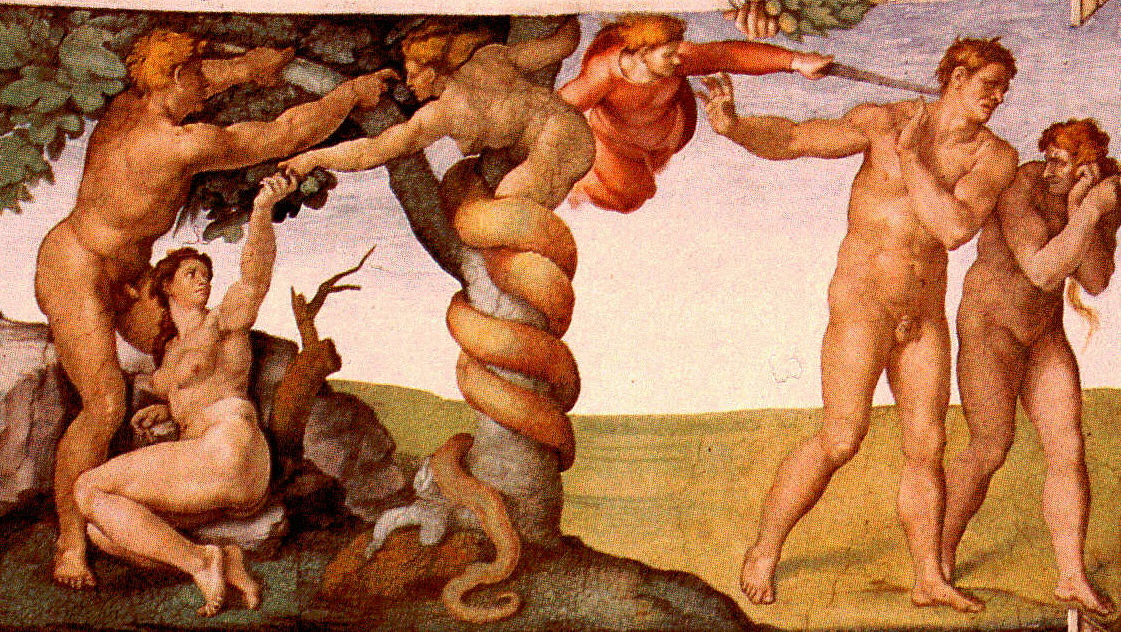
\includegraphics[width=\textwidth]{../../../graphics/the_fall.jpg}
\end{frame}

% section kant_s_three_propositions (end)

\section{Next Time}\label{sec:next_time} % (fold)

\emph{Groundwork} \S 2.

\begin{frame}<presentation>[label=slide12]
    \frametitle{Reading for Next Time}
        \begin{columns}
            \begin{column}{3cm}
                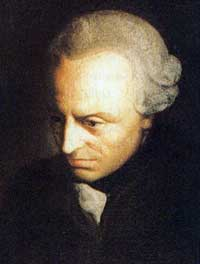
\includegraphics[height=4cm]{../../../graphics/kant.jpg}
            \end{column}
            \begin{column}{7cm}
                \alert{Groundwork \S 2}
            \end{column}
        \end{columns}
\end{frame}

% section next_time (end)

\end{document}
